\documentclass[a4paper]{article}
\usepackage[spanish]{babel}
\usepackage[utf8]{inputenc}
\usepackage{charter}   % tipografia
\usepackage{graphicx}
%\usepackage{makeidx}
\usepackage{paralist} %itemize inline
\usepackage{pdfpages}


%\usepackage{float}
%\usepackage{amsmath, amsthm, amssymb}
%\usepackage{amsfonts}
%\usepackage{sectsty}
%\usepackage{charter}
%\usepackage{wrapfig}
%\usepackage{listings}
%\lstset{language=C}


\usepackage{color} % para snipets de codigo coloreados
\usepackage{fancybox}  % para el sbox de los snipets de codigo

\definecolor{litegrey}{gray}{0.94}

% \newenvironment{sidebar}{%
% 	\begin{Sbox}\begin{minipage}{.85\textwidth}}%
% 	{\end{minipage}\end{Sbox}%
% 		\begin{center}\setlength{\fboxsep}{6pt}%
% 		\shadowbox{\TheSbox}\end{center}}
% \newenvironment{warning}{%
% 	\begin{Sbox}\begin{minipage}{.85\textwidth}\sffamily\lite\small\RaggedRight}%
% 	{\end{minipage}\end{Sbox}%
% 		\begin{center}\setlength{\fboxsep}{6pt}%
% 		\colorbox{litegrey}{\TheSbox}\end{center}}

\newenvironment{codesnippet}{%
	\begin{Sbox}\begin{minipage}{\textwidth}\sffamily\small}%
	{\end{minipage}\end{Sbox}%
		\begin{center}%
		\vspace{-0.4cm}\colorbox{litegrey}{\TheSbox}\end{center}\vspace{0.3cm}}



\usepackage{fancyhdr}
\pagestyle{fancy}

%\renewcommand{\chaptermark}[1]{\markboth{#1}{}}
\renewcommand{\sectionmark}[1]{\markright{\thesection\ - #1}}

\fancyhf{}

\fancyhead[LO]{Sección \rightmark} % \thesection\ 
\fancyfoot[LO]{\small{Aldasoro Agustina, Bouz\'on Mar\'ia Bel\'en, Cairo Gustavo Juan}}
\fancyfoot[RO]{\thepage}
\renewcommand{\headrulewidth}{0.5pt}
\renewcommand{\footrulewidth}{0.5pt}
\setlength{\hoffset}{-0.8in}
\setlength{\textwidth}{16cm}
%\setlength{\hoffset}{-1.1cm}
%\setlength{\textwidth}{16cm}
\setlength{\headsep}{0.5cm}
\setlength{\textheight}{25cm}
\setlength{\voffset}{-0.7in}
\setlength{\headwidth}{\textwidth}
\setlength{\headheight}{13.1pt}

\renewcommand{\baselinestretch}{1.1}  % line spacing


% \setcounter{secnumdepth}{2}
\usepackage{underscore}
\usepackage{caratula}
\usepackage{url}




\begin{document}


\thispagestyle{empty}
\materia{M\'etodos Num\'ericos}
\submateria{Segundo Cuatrimestre de 2014}
\titulo{Trabajo Práctico III}
\subtitulo{Develando la mentira de los megap\'ixeles}
\integrante{Aldasoro Agustina}{86/13}{agusaldasoro@gmail.com}
\integrante{Bouz\'on Mar\'ia Bel\'en}{128/13}{belenbouzon@hotmail.com}
\integrante{Cairo Gustavo Juan}{89/13}{gjcairo@gmail.com}

\maketitle
\newpage

\thispagestyle{empty}
\vfill
\begin{abstract}
En el presente trabajo se pretende analizar y comparar distintas alternativas que pretenden dar respuesta al problema de demosaicing. Para ello, las mismas serán implementadas y sometidas a experimentación sobre fotografías crudas sintéticas específicamente seleccionadas para poner de manifiesto las ventajas e inconvenientes del empleo de cada método. \\
\end{abstract}

\textbf{Palabras clave:} \\
$\bullet$ Filtro Bayer \\
$\bullet$ Demosaicing \\
$\bullet$ Interpolaci\'on \\
$\bullet$ Artifacts \\



\thispagestyle{empty}
\vspace{3cm}
\tableofcontents
\newpage


%\normalsize
\newpage

\section{Introducci\'on Te\'orica}

Promediando la década de 1990 comenzaron a introducirse al mercado las cámaras digitales de uso hogareño, empezando a sustituir desde entonces a las ampliamente difundidas cámaras de film. 
Mientras que estas últimas capturaban la imagen de forma mecánica y sin intercesión de un procesamiento digital (\textcolor{red}{¿? Asegurarse cómo es y explayarse. Estuve buscando y no entendi o no encontre nada. me parece que asi esta bien}), las cámaras electrónicas emplearon una nueva tecnología. Esta tecnolog\'ia distingue entre en el momento de obtención de un conjunto de datos cerca del objetivo – donde se obtiene una imagen que llamaremos “\textit{cruda}” – y una etapa de procesamiento automático conjunto a la reconstrucción de la imagen final. \\

En el presente trabajo nos interesará analizar un fragmento de dicha etapa conocido como \emph{demosaicing}. Para entender de qué consta, es menester comprender previamente la forma en que se capturan las imágenes al utilizar cámaras digitales.

Este tipo de cámaras poseen un sensor CCD compuesto de una matriz de elementos fotosensibles, cada uno de los cuales es capaz de captar la intensidad de la luz que llega a ese punto a través de la lente. 

La tarea de capturar todos los colores reflejados por el objetivo que se quiere fotografiar no está encomendada a ninguna posición en particular, sino que cada una de ellas tiene asignada – de acuerdo a algún patrón definido  – la captura de la información perteneciente a un solo color. Cada p\'ixel de la imagen va a estar dividido en tres canales ya que la vamos a almacenar mediante RGB (Red, Green, Blue).

El patr\'on que determina qué color será capturado por cada fotosensor es denominado \emph{Color Filter Array} y var\'ia de acuerdo al fabricante de c\'amaras. Existen diversos patrones, en nuestro trabajo nos centraremos en el \textbf{Filtro Bayer}, ya que es un filtro com\'unmente usado debido a que la cantidad de informaci\'on que brinda sobre el canal verde - al cual el ojo humano es más sensible -.

\textcolor{blue}{*insertar imágenes por aquí y por allá*:\\
Filtro Bayer \\
Otros filtros (?
}

\begin{figure}[h!]
	\caption{Bayer CFA}
	\begin{center}
	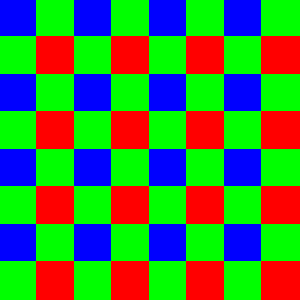
\includegraphics[scale=0.36]{imagenes/BayerFilter}
	\label{Bayer}
  \end{center}
\end{figure}


%, a causa de que se encuentra en el centro de su espectro visual - duplica a cada uno de los otros dos. 

Ahora bien, esto genera una imagen que se aproxima a la realidad sólo en parte ya que para cada p\'ixel de la imagen tenemos la informaci\'on de s\'olo uno de sus tres canales. A causa de esto es que la misma debe ser reconstruida algorítmicamente, interpolando los valores de los colores que no fueron almacenados explícitamente para cada pixel.


En este punto adquieren relevancia las diferentes propuestas de reconstrucción de la imagen original. Esto conlleva la ejecución de diversos procedimientos, entre los que se encuentran el demosaicing, el análisis del balance de blancos, la curva tonal, la saturación y el contraste y la compresión final de la imagen. Como nuestra propuesta se aboca al primer paso mencionado, exploraremos en el presente trabajo sólo un subconjunto de una serie de variaciones no finita que admiten métodos de debayering como ser la interpolación por asignación de valores próximos, la interpolación bilineal y interpolación direccional.\\

\newpage
\subsection{Inconvenientes de aproximar mediante el Polinomio de Lagrange}

\textcolor{blue}{Arreglar un poco las refs}

Es nuestra intención exponer ahora el motivo que consideramos suficiente para decidir interpolar los valores ausentes a través de Splines en lugar de hacer uso del polinomio de Lagrange.\\
Sea dada la siguiente muestra: \\
\smallskip


\begin{tabular}{ | c || c | c | c | c | c |c | c | c | c | c | c | c | c | c | c |}
 \hline                 
   x & 1 & 2 & 3 & 4 & 5 & 6 & 7 & 8 & 9 & 10 & 11 & 12 & 13 & 14 \\
 \hline    
y & 10 & 10 & 10& 10& 10& 10& 10& 10& 10& 10& 10& 10& 10& 10 \\
 \hline  
 \end{tabular}

\smallskip

\begin{tabular}{  | c || c | c | c | c | c |c | c | c | c | c | c | c | c | c | c |}
 \hline                 
   x&15& 16 & 17 & 18 & 19 & 20 & 21 & 22 & 23 & 24 & 25 & 26 & 27 & 28\\
 \hline    
y & 10 & 10 & 10& 10& 10& 10& 10& 10& 10& 10& 10& 10& 10& 10 \\
 \hline  
 \end{tabular}
\smallskip
\\
El polinomio de Lagrange que interpola cada uno de esos valores tiene una expresión equivalente al Spline que lo hace, siendo su gráfico el citado a continuación:
\smallskip

\begin{figure}[h!]
	\caption{}
	\begin{center}
	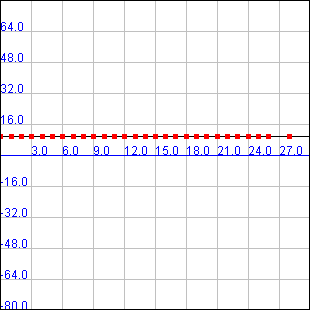
\includegraphics[scale=1]{imagenes/LagrangeSplinesCTE}
	\label{LagrangeSplinesCTE}
  \end{center}
\end{figure}

Supongamos ahora que el resultado de una medición - digamos $x_{12}$ - haya sido calculada con un ruido que represente el 1\% del valor real, modificándose la muestra de la siguiente forma:\\

\smallskip

\begin{tabular}{ | c || c | c | c | c | c |c | c | c | c | c | c | c | c | c | c |}
 \hline                 
   x & 1 & 2 & 3 & 4 & 5 & 6 & 7 & 8 & 9 & 10 & 11 & 12 & 13 & 14 \\
 \hline    
y & 10 & 10& 10& 10& 10& 10& 10& 10& 10& 10& 10& 10,1& 10 & 10\\
 \hline  
 \end{tabular}

 \smallskip

\begin{tabular}{  | c || c | c | c | c | c | c | c | c | c | c | c | c | c | c | }
 \hline                 
   x&15& 16 & 17 & 18 & 19 & 20 & 21 & 22 & 23 & 24 & 25 & 26 & 27 & 28\\
 \hline    
y & 10 & 10 & 10& 10& 10& 10& 10& 10& 10& 10& 10& 10& 10& 10 \\
 \hline  
 \end{tabular}

\smallskip
 En este caso se obtendría el gráfico representado en la Figura \ref{LagrangeX12a101} para el polinomio de Lagrange (escalado en la Figura \ref{LagrangeX12a101(zoomOut)})y el que se ilustra en la Figura \ref{SplinesX12a101} para el obtenido mediante Splines.\\

\begin{figure}[h!]
	\caption{}
	\begin{center}
	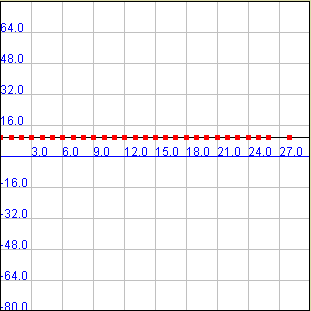
\includegraphics[scale=1]{imagenes/SplinesX12a101}
	\label{SplinesX12a101}
  \end{center}
\end{figure}

\begin{figure}
	\caption{}
	\begin{center}
	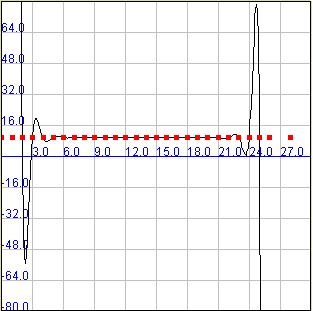
\includegraphics[scale=1]{imagenes/LagrangeX12a101}
	\label{LagrangeX12a101}
  \end{center}
\end{figure}

\begin{figure}
	\caption{}
	\begin{center}
	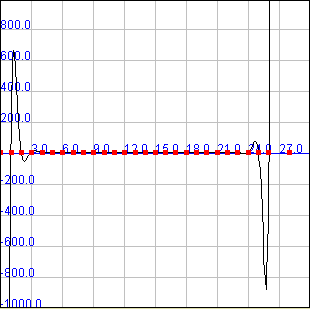
\includegraphics[scale=1]{imagenes/LagrangeX12a101(zoomOut)}
	\label{LagrangeX12a101(zoomOut)}
  \end{center}
\end{figure}

Como se puede observar, para la construcción del Spline el cambio en un valor de la imagen no impactó de una forma apreciable sobre el resto del polinomio. Sin embargo, el nuevo resultado generó un polinomio de Lagrange cuya diferencia con la Figura \ref{SplinesX12a101} es grosera en determinados intervalos.\\ 

Si se profundizara el error de la medición de acuerdo con la tabla presentada a continuación, notaríamos que el polinomio de Lagrange comenzaría a presentar una mayor cantidad de intervalos con valores drásticamente alejados de los dados como referencia. Por otro lado, Splines únicamente presentará variaciones en un entorno de los intervalos cuyos valores hayan sido modificados. Esto se puede  constatar en las Figuras \ref{SplinesX12a20}, \ref{LagrangeX12a20} y  \ref{LagrangeX12a20(zoomOut)}.\\


\begin{tabular}{ | c || c | c | c | c | c |c | c | c | c | c | c | c | c | c | c |}
 \hline                 
   x & 1 & 2 & 3 & 4 & 5 & 6 & 7 & 8 & 9 & 10 & 11 & 12 & 13 & 14 \\
 \hline    
y & 10 & 10& 10& 20& 10& 10& 10& 10& 10& 10& 10& 20& 10 & 10\\
 \hline  
 \end{tabular}

\smallskip

\begin{tabular}{  | c || c | c | c | c | c | c | c | c | c | c | c | c | c | c | }
 \hline                 
   x&15& 16 & 17 & 18 & 19 & 20 & 21 & 22 & 23 & 24 & 25 & 26 & 27 & 28\\
 \hline    
y & 10 & 10 & 10& 10& 10& 10& 10& 10& 10& 10& 10& 10& 10& 10 \\
 \hline  
 \end{tabular}

\begin{figure}
	\caption{}
	\begin{center}
	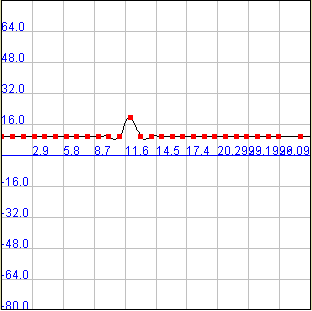
\includegraphics[scale=1]{imagenes/SplinesX12a20}
	\label{SplinesX12a20}
  \end{center}
\end{figure}

\begin{figure}
	\caption{}
	\begin{center}
	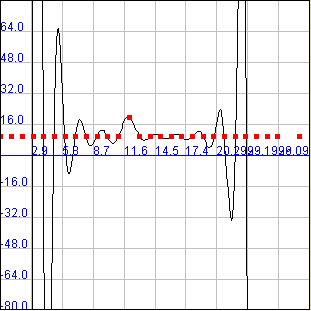
\includegraphics[scale=1]{imagenes/LagrangeX12a20}
	\label{LagrangeX12a20}
  \end{center}
\end{figure}

\begin{figure}
	\caption{$Zoom \ out$ de la Figura \ref{LagrangeX12a20}}
	\begin{center}
	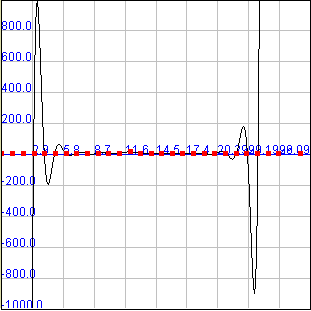
\includegraphics[scale=1]{imagenes/LagrangeX12a20(zoomOut)}
	\label{LagrangeX12a20(zoomOut)}
  \end{center}
\end{figure}


En conclusión, el polinomio de Lagrange se comporta de una manera menos predecible \textcolor{red}{en realidad sí es predecible si tenés el polinomio y podés evauarlo, pero quiero decir q es menos intuitivo, menos "constante", como que hace cualquiera entre dos puntos cuya imagen no esté fijada de antemano} entre dos variables independientes y no garantiza que en esos intervalos el valor de la función sea cercano a los ya conocidos.\\
La carencia de predictibilidad hace del polinomio de Lagrange una mala alternativa para la interpolación, en comparación con las ventajas proporcionadas por el empleo de Splines.\\


\newpage
\subsection{Artifacts}
\textcolor{blue}{Aca explicar un poco que onda,  que son los artifacts}

\newpage
\section{Desarrollo}

Dada una \textit{imagen cruda}, los valores que contiene en sus píxeles para cada canal los asumimos reales y ciertos. Por lo tanto, resta averiguar para cada uno de ellos los valores de los dos canales para los cuales dicha información se encuentra ausente.

\subsection{Vecino m\'as cercano}
La implementación más sencilla para la estimación de los canales desconocidos de cada pixel consiste en otorgar a cada canal ``vacío'' el valor real m\'as pr\'oximo que corresponda a dicho color. Este m\'etodo es algor\'itmicamente asequible, pero no tiene en cuenta dos factores: \\
\\

$\triangleright$ Por un lado, al otorgar el valor de un sólo pixel cercano, surge la necesidad de definir arbitrariamente cuál se debe escoger como valor referencial en casos en que un conjunto de pixeles son equidistantes al analizado y no existe un criterio claro acerca de cuál de ellos debe ser considerado el ``más próximo''. Que esta decisión impacte en el resultado de forma inocua o parcial o totalmente nociva dependerá en cierta medida de la fotografía que se esté analizando.

El ejemplo más trivial se encuentra en una imagen monocromática: al ser los valores reales idénticos para todos los pixeles, tomar las magnitudes de cualquier otra posición para cada canal correspondiente no afectará el resultado final. Sin embargo, si consideráramos una imagen formada por columnas alternadas de un pixel de ancho rojas (\#0000FF) y blancas (\#FFFFFF), entonces si para definir los canales verde y azul de un pixel rojo se tomara como posiciones más cercanas aquel que se encuentra debajo suyo y el que está a la derecha del mismo (respectivamente), el resultado sería un pixel fucsia (\#FF00FF). En cambio, si los pixeles elegidos fueran su inmediato derecho y en el que se encuentra a su diagonal inferior derecha, la posición analizada debería manifestar el color blanco (\#000000).

Si bien se trata de un ejemplo de alcance limitado, resulta suficiente para ilustrar los potenciales problemas de la aplicación de este algoritmo.\\

\textcolor{blue}{Aca va la fotito que tiene que armar Belu}\\

$\triangleright$ Por otra parte - y en cierta forma vinculado al ejemplo anterior - este método no especifica ninguna distinción respecto de la forma de proceder en casos de borde o de superficies parejas. \\


\newpage
\subsection*{Decisiones tomadas en el Algoritmo de Vecino M\'as Cercano}

A la hora de formular nuestro algoritmo de Vecino m\'as Cercano nos vimos obligados a determinar aspectos que conciernen al dise\~no del mismo. 

La principal decisi\'on que debimos tomar fue con qu\'e criterio elegir al p\'ixel m\'as cercano cuando no es \'unico (esto ocurre en todos los casos). 

\begin{figure}[h!]
	\caption{}
	\begin{center}
	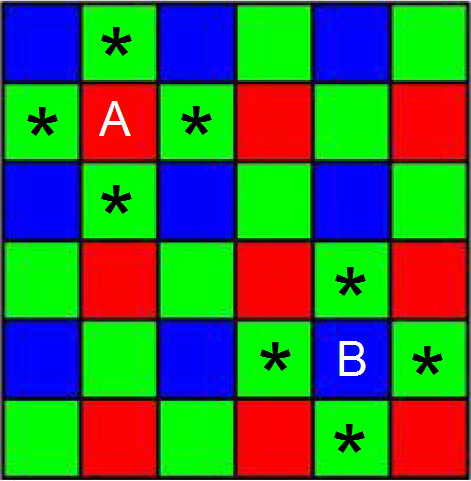
\includegraphics[scale=0.36]{imagenes/vecino1}
	\label{Vecino1}
  \end{center}
\end{figure}

Para determinar el valor del canal verde sobre un p\'ixel definido rojo\emph{(A)} o azul\emph{(B)} tenemos cuatro p\'ixeles a la misma distancia (1) que nos brindan informaci\'on sobre el canal verde. 
\begin{figure}[h!]
	\caption{}
	\begin{center}
	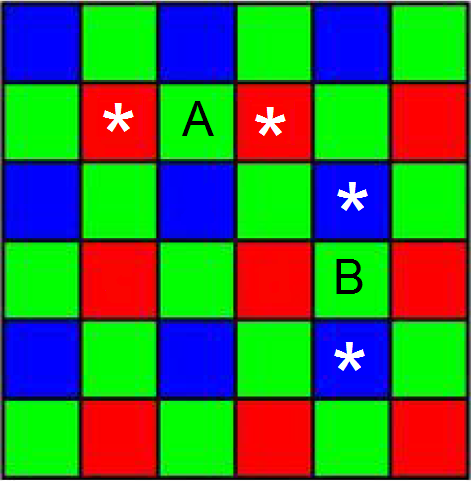
\includegraphics[scale=0.36]{imagenes/vecino2}
	\label{Vecino2}
  \end{center}
\end{figure}

Si nos situamos en un p\'ixel naturalmente verde, tanto para determinar su canal rojo\emph{(A)} como para determinar su canal azul\emph{(B)} sus p\'ixeles m\'as cercanos que nos brindan informaci\'on son dos (a 1 de distancia cada uno). 
\begin{figure}[h!]
	\caption{}
	\begin{center}
	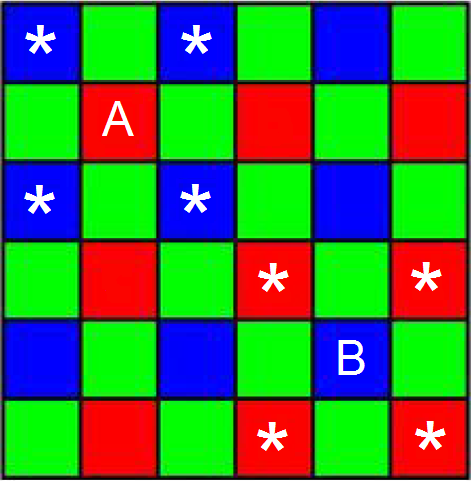
\includegraphics[scale=0.36]{imagenes/vecino3}
	\label{Vecino3}
  \end{center}
\end{figure}

Y por \'ultimo para determinar el valor del canal azul sobre un p\'ixel de origen rojo\emph{(A)} (y viceversa\emph{(B)}) nos encontramos con cuatro p\'ixeles a la misma m\'inima distancia (2) en sus diagonales. \\

Por este motivo, realizamos dos versiones de este algoritmo variando en ellas cu\'al p\'ixel elegir para rellenar el canal verde cuando se est\'a situado sobre un p\'ixel azul o rojo.

En el \emph{\textbf{algoritmo 1}} si se est\'a en un p\'ixel rojo se elige al de arriba y si se est\'a en un p\'ixel azul se elige el de la derecha. En cambio, en el \emph{\textbf{algoritmo 2}} si se est\'a en un p\'ixel rojo se elige al de la izquierda y si se est\'a en un p\'ixel azul se elige al de abajo.

Corrimos ambos algoritmos con diversas fotos, a continuaci\'on se muestran algunos ejemplos:

\begin{figure}[h!]
	\caption{}
	\begin{center}
	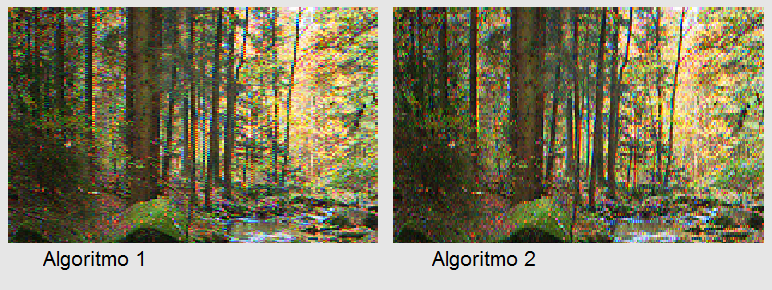
\includegraphics[scale=0.60]{imagenes/Vecino/arbolitos}
	\label{arbolitos}
  \end{center}
\end{figure}

\begin{figure}[h!]
	\caption{}
	\begin{center}
	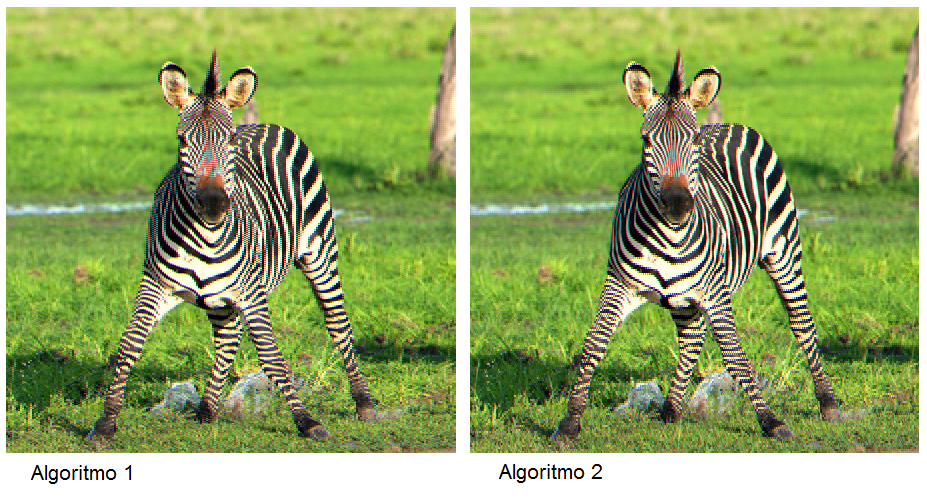
\includegraphics[scale=0.60]{imagenes/Vecino/zebraCara}
	\label{zebraCara}
  \end{center}
\end{figure}

\newpage
\begin{figure}[h!]
	\caption{}
	\begin{center}
	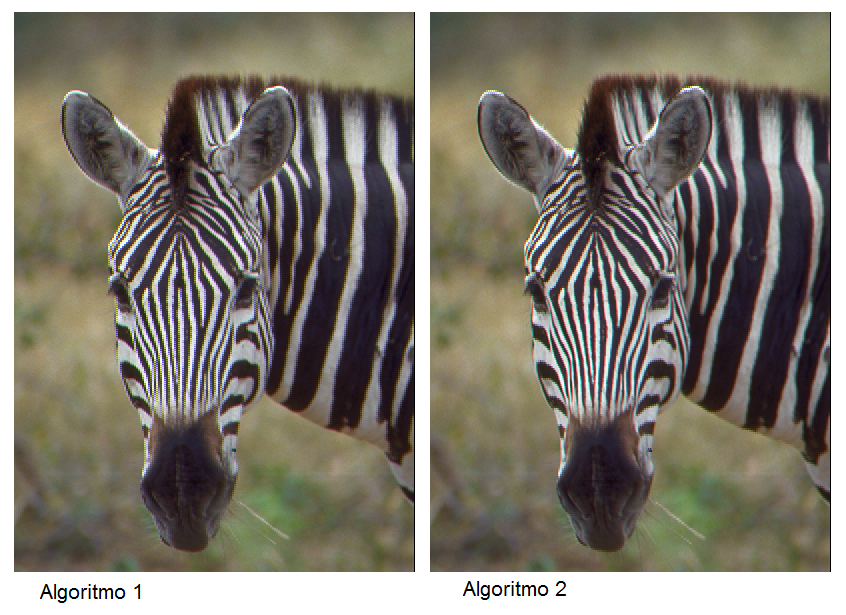
\includegraphics[scale=0.60]{imagenes/Vecino/zebra}
	\label{Zebra}
  \end{center}
\end{figure}

Se puede apreciar que el Algoritmo 1 es capaz de delimitar mejor bordes que poseen rayas en forma horizontal, en cambio el Algoritmo 2 le da una mejor definici\'on a los bordes verticales. Dada la forma de la implementaci\'on, las anomal\'ias observadas en las imagenes cobran sentido.\\

\textcolor{blue}{ACA falta poner el psnr y el ssim}

Dado a que no se puede establecer con un criterio cu\'al es m\'as correcta que la otra, ya que la veracidad de la imagen obtenida var\'ia depende la imagen inicial y su estructura. Nosotros optamos por utilizar el \emph{\textbf{Algoritmo 1}}.

Se adjuntan las im\'agenes en su tama\~no original. \textcolor{red}{ADJUNTARLAS!!!!!!!!}

\newpage
\subsection{Interpolaci\'on Bilineal}

La interpolación bilineal es una composición de interpolaciones lineales en dos direcciones diferentes. Este método desmerece el caracter arbitrario de asignación de un canal a partir del valor más próximo para el mismo y propone que el resultado final sea calculado teniendo en cuenta y promediando todos los valores cercanos sin priorizar ninguno de ellos. \\

Como la estructura del filtro Bayer sólo asegura para los p\'ixels nativamente azules o rojos tener todas sus posiciones vecinas netamente verdes, aquel es el único caso en que el cálculo de un canal se reduce a computar el promedio de los valores superior, inferior, derecho e izquierdo al espacio que se quiere interpolar.

Sin embargo, si se quisiera obtener el valor de azul o rojo que correspondería asignar a un pixel nativamente verde, el entramado de Bayer obligaría a estimarlo a partir de sus dos valores m\'as cercanos ubicados a la derecha e izquierda o arriba y abajo dependiendo de la ubicaci\'on del p\'ixel. 

Por otro lado, los valores del canal azul para un pixel rojo (y los del canal rojo para un pixel azul) se calcularían tomando en cuenta las cuatro posiciones diagonales a la analizada. Este proceso no se realizar\'ia simplemente tomando el promedio de sus cuatro diagonales sino que requeriría tomar dos pixels cercanos que pertenezcan a la misma fila o columna, cuyo canal real sea el verde, calcular sus valores de azul/rojo promediando los de las casillas nativas azules/rojas más próximas y posteriormente realizar un nuevo promedio entre los valores resultantes.

Tomando como referencia la ilustración \ref{bilineal} se puede ver que el cálculo recien descripto equivale a calcular el valor en el canal rojo para el p\'ixel x. Lo cual consistir\'ia en: 

Hacer el promedio entre \textit{a y b} y luego, ubicar ese valor para el canal rojo para el p\'ixel ubicado arriba de x.

Hacer el promedio entre \textit{c y d} y luego, ubicar ese valor para el canal rojo para el p\'ixel ubicado debajo de x.

Una vez obtenidos estos dos valores, promediarlos y ubicarlos en el canal rojo de x.\\

Llegando as\'i a que realizar este c\'alculo es equivalente a realizar el promedio entre los valores de sus diagonales:

\[
 \frac{a+b}{2} + \frac{c+d}{2} = \frac{a+b+c+d}{4}
\]

\begin{figure}[h!]
	\caption{}
	\begin{center}
	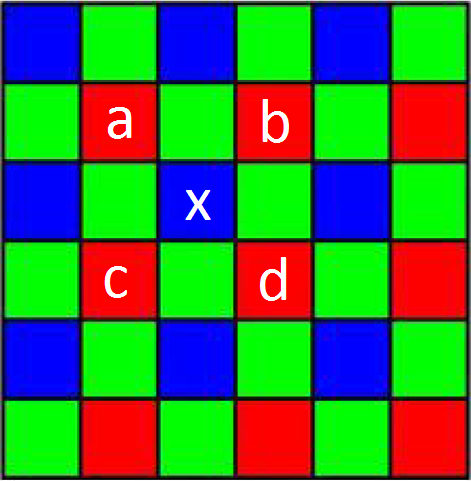
\includegraphics[scale=0.36]{imagenes/bilineal}
	\label{bilineal}
  \end{center}
\end{figure}

\newpage
\subsection{Interpolaciones Direccionales}
Se trata de una gran cantidad de métodos que buscan comenzar a resolver el problema de demosaicing realizando inicialmente una interpolación en una dirección y combinando con algún criterio determinado el resultado estimado con el obtenido de una aproximación realizada en otra dirección.\\

La implementación de este tipo de métodos exige tomar al menos dos decisiones de peso que distinguirán a unos de otros:\\

\begin{itemize}
    \item De qué forma se realizarán las interpolaciones (en qué direcciones y mediante qué mecanismo de interpolación)
    \item Con qué criterio y consideraciones combinar la información proporcionada por las direcciones escogidas.
\end{itemize}

Para escoger alguna opción apropiada corresponde analizar las características del Color Filter Array con el que se va a trabajar, puesto que no todas las direcciones van a aportar en la totalidad de los casos la misma información.

En cuanto a la combinación de los resultados de las distintas interpolaciones, es conveniente tener presente que el promedio de los mismos no es siempre una buena opción. Por ejemplo, supongamos que se analiza una imagen que presenta en un sector las características observables en la Imagen original de la ilustración \ref{apxl1}.


\begin{figure}[h!]
	\caption{}
	\begin{center}
	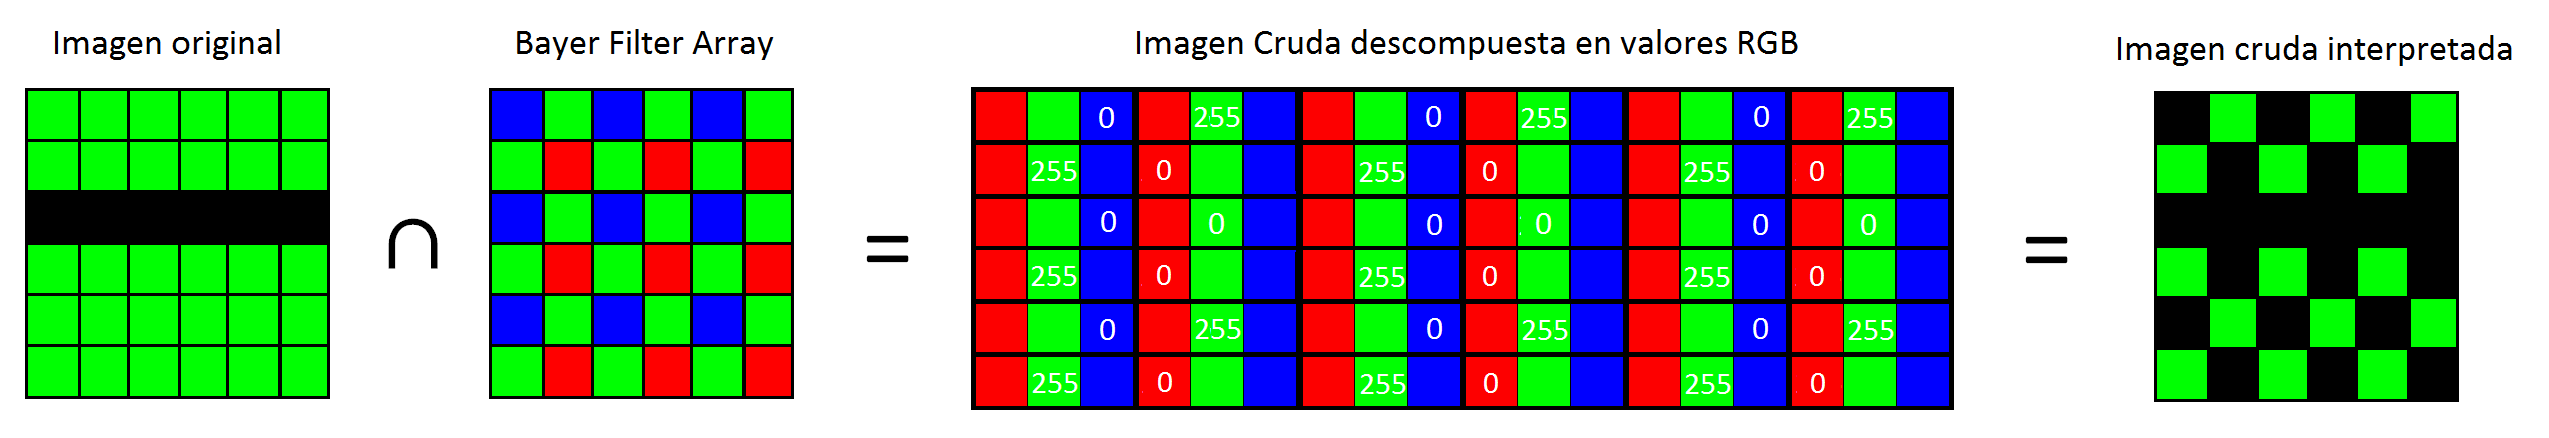
\includegraphics[scale=0.36]{imagenes/apxl1}
	\label{apxl1}
  \end{center}
\end{figure}

En dicha figura se analiza la información de la misma que sería captada por los fotosensores respondiendo al Bayer Filter Array. 

En el esquema \ref{apxl2} se puede observar que para varios pixeles la interpolación horizontal retorna valores distintos a la realizada verticalmente (esto tiene sentido, pues se trata de un área homogénea atravesada por una fila de distinto color).

El resultado de empleo del promedio como estrategia de nivelacion de dichos valores queda expuesto en la Figura \ref{apxl3}, en la cual se puede observar el causante del artifact \"zipping\", producto de un algoritmo indiferente ante los cambios de color abruptos.\\

\begin{figure}[h!]
	\caption{}
	\begin{center}
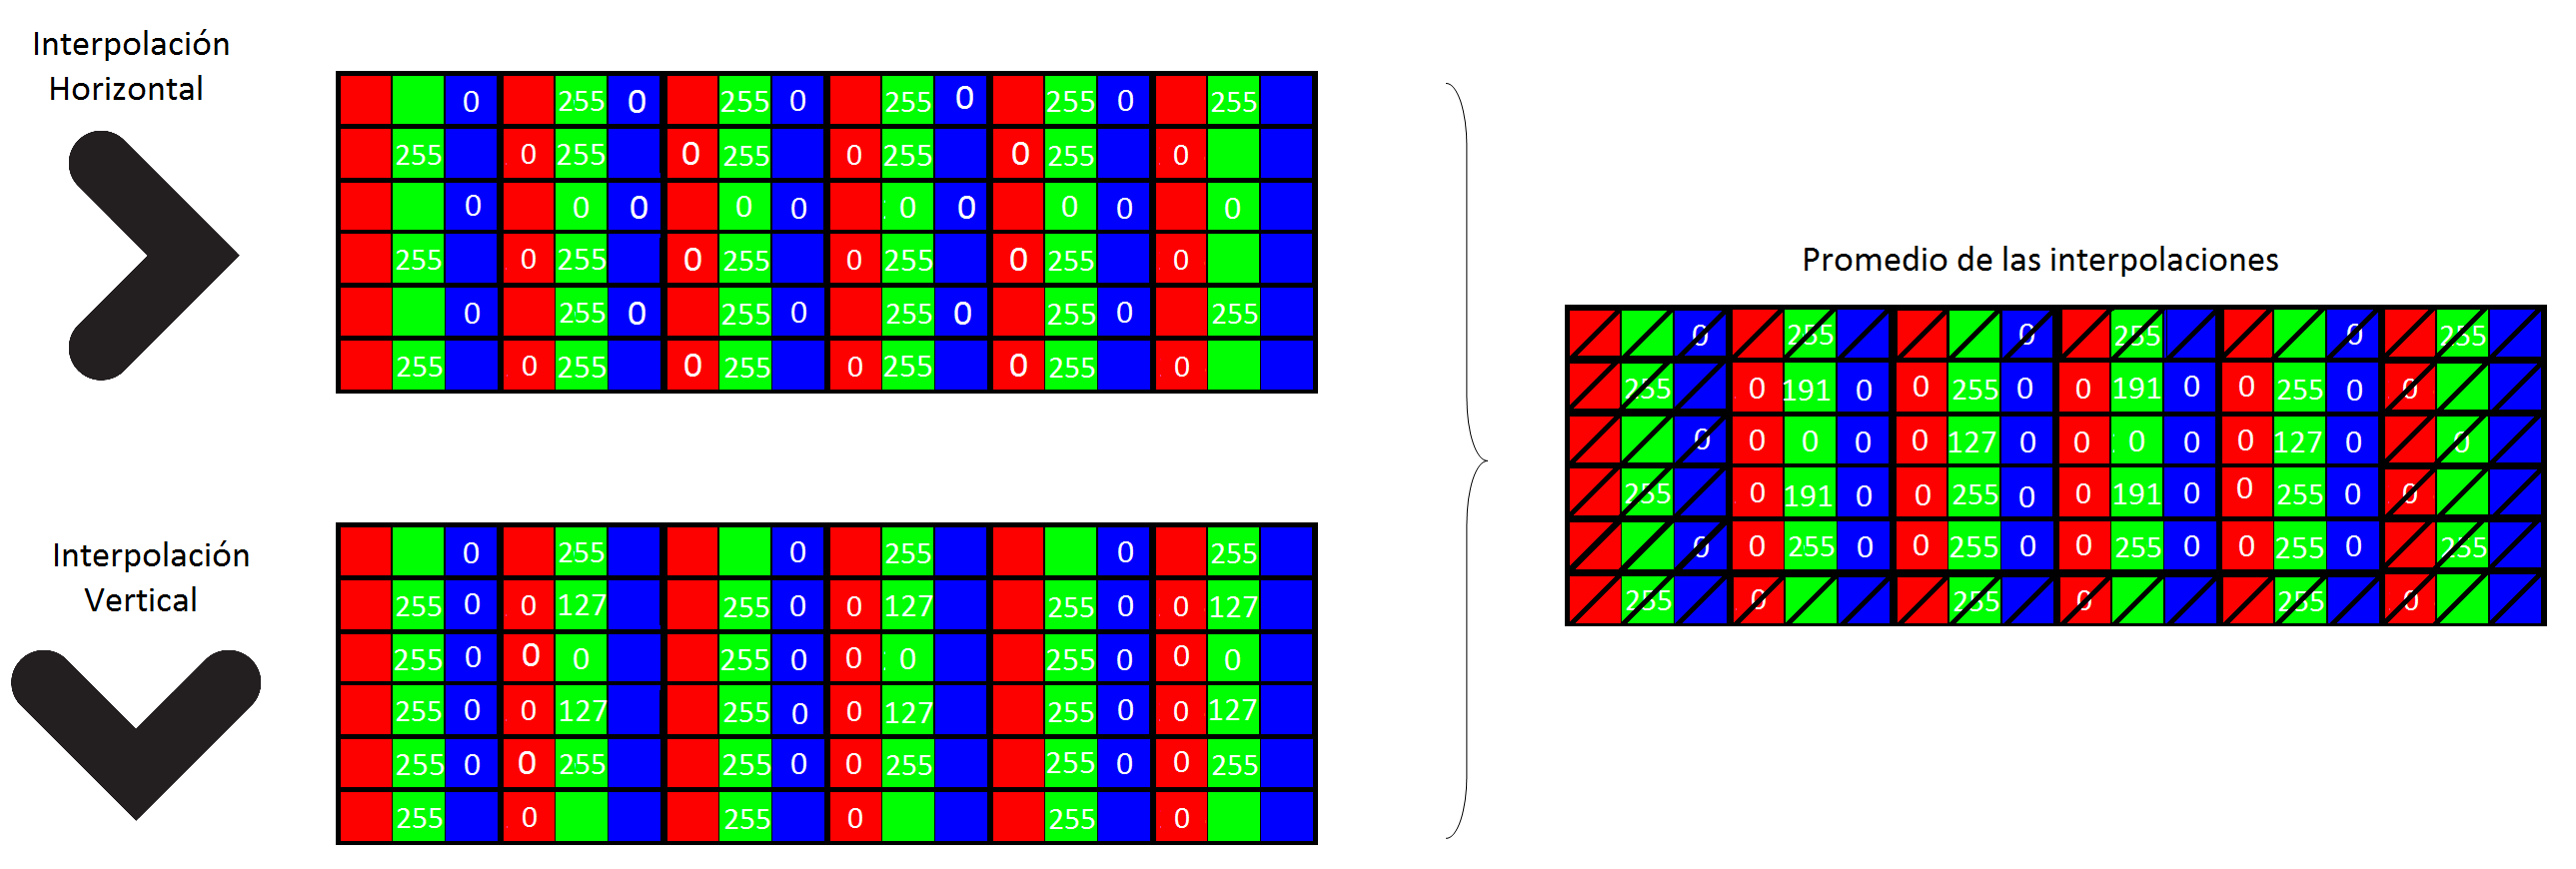
\includegraphics[scale=0.26]{imagenes/apxl2}
	\label{apxl2}
  \end{center}
\end{figure}

\begin{figure}[h!]
	\caption{}
	\begin{center}
	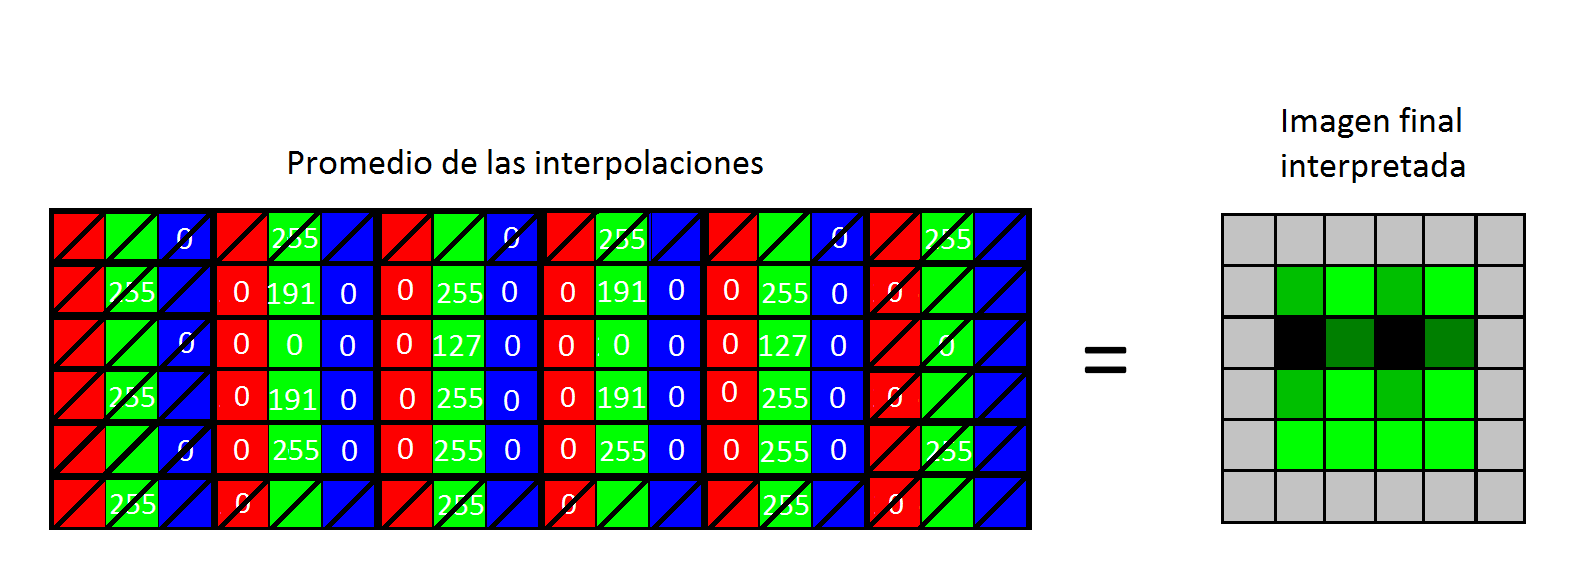
\includegraphics[scale=0.36]{imagenes/apxl3}
	\label{apxl3}
  \end{center}
\end{figure}

Ciertamente esto no es lo esperado y existen mecanismos que permiten corregir este error. Uno de ellos consiste en calcular el gradiente del color para utilizarlo al combinar los resultados, de modo tal que si el mismo fuera de gran magnitud (es decir, la variación del color es considerable) entonces el peso que debe tener el valor calculado en el resultado final debería ser menor a aquel que fue calculado en una dirección cuyo gradiente fuera menor (es decir, que se tratara de una superficie más cromáticamente homogénea).



\pagebreak

\subsection*{Versiones de Splines}

\textcolor{blue}{Hablar de todos sus tipos\\
Decir que bilineal y poner 0.5 queda igual (o casi igual je), usar psnr.\\
Y ver cual vamos a dejar\\
Y que usamos NATURALES}

\newpage
\subsection{Algoritmo de Malvar, He y Cutler}
\textcolor{blue}{Hablar un poco aca del paper...}
\newpage
\subsection{Exploraci\'on de Artifacts}

\textcolor{blue}{Ver si hay otros artifacts mas para agregar.\\
Ver como arreglar el de Moire y bla...\\
Poner fotitos de ampliaciones donde se vean bien los artifacts.}


\newpage
\section{Resultados y discusi\'on}

\newpage
\subsection{MHC}
Le da muchísima más definición/claridad a las fotos, y los bordes oscuros quedan prácticamente perfectos (comparando con bilineal, por ejemplo, aparecen colores fuertes alrededor de los bordes negros). Sigue pasando eso con los bordes blancos/mas claros, pero las zonas donde hay un salto grande entre claro y oscuro, mejora mucho.

\newpage
\subsection{An\'alisis cualitativo de los algoritmos}
Luego de haber generado las im\'agenes con todos los algoritmos que hemos propuesto, nos dispusimos a correr en Matlab$\textregistered$  la diferencia entre ellas y la imagen original de la cual partimos. Luego de eso, invertimos los colores para poder apreciar mejor d\'onde se notaban las mayores diferencias. A continuaci\'on se incluyen las im\'agenes obtenidas con este proceso, en color blanco y negro.\\

\textcolor{blue}{Aca falta agregar todas las fotitos, Y HACERLO PARA SPLINES!!!!!!!!!!!!!!!!!}
%ESTO PUEDE IR DE PIE DE IMAGEN O ALGO ASI...
%De este modo, en los siguientes gr\'aficos se denotan los lugares con diferencia num\'erica de la imagen.


En la "imagen 2"  se puede observar que, si bien al ejecutar el algoritmo de MHC disminuye abundantemente la diferencia con la imagen original, al tener una superficie en su mayor\'ia de agua se dificulta a niveles algor\'itmicos aproximar el agua de una manera m\'as real ya que esta no es para nada una superficie pareja. \textcolor{red}{(SI EXPLICO EL PORQUE PASA ESTO, MANDO FRUTA ASI QUE NO VOY A HACERLO)'.}\\

En la "imagen 4" se puede apreciar el inconveniente de aproximar p\'ixeles que son borde cuando estos son dados en abundancia y en l\'ineas recta en su mayor\'ia. Inclusive en el mejor caso de esta imagen, (la imagen creada mediante el Algoritmo de MHC) se puede apreciar una notable diferencia con la original en lo que respecta a los bordes. \textcolor{red}{Esto es un ejemplo m\'as de la existencia de artifacts.}\\

En cuanto a la "imagen 5" se aprecia el mismo inconveniente que en la "imagen 1" dado a la existencia de agua, pero a diferencia cuando se corre el algoritmo de MHC la mejor\'ia es notablemente mayor ya que la diferencia entre esta imagen y la foto original es muy peque\~na.\\

En la "imagen 9" se puede ver un comportamiento similar a lo ya estudiado, lo interesante de destacar en cuanto a esta foto es que al poseer un letrero es una imagen menos abstracta que las anteriores y por lo tanto, se adquiere una definici\'on mayor cuando se tiene una diferencia menor con la original y as\'i facilitar la lectura del cartel.


\begin{figure}[h!]
	\caption{}
	\begin{center}
	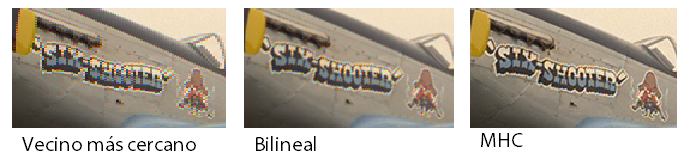
\includegraphics[scale=0.05]{imagenes/comparacion/cartel}
	\label{cartel}
  \end{center}
\end{figure}


La "imagen 12" es una imagen con muchas l\'ineas y dibujos con contornos esto se aprecia en la gran densidad que tiene la imagen que muestra las diferencias entre la imagen original y la imagen obtenida mediante el algoritmo de Vecino M\'as Cercano. Si observamos las im\'agenes obtenidas mediante la resta con sus respectivas originales se denota una gran diferencia entre el Algoritmo de Vecino M\'as Cercano y el Algoritmo de MHC.\\

Como conclusi\'on, podemos inferir que los lugares donde se muestra una variaci\'on son siempre lugares pertencientes a contornos o bordes de objetos en las im\'agenes. En cambio, en p\'ixeles sobre superficies llanas o parejas del mismo cuerpo la diferencia entre la imagen original y nuestra imagen obtenida es nula.


\subsection{An\'alisis de tiempos}
\textcolor{blue}{Aca hay que comparar los tiempos de ejecucion entre todos los algoritmos dispuestos.}

\newpage
\section{Conclusiones y trabajo futuro}





\section{Ap\'endices}
\subsection{Ap\'endice A: Enunciado} 

%ACORDARSE DE DESCOMENTARLO%%%%%%%%%%%%%%%%%%%%%%%%%%%%%%%%%%%%%%%%%%%%%%%%%%%%%%%%%%%%%

%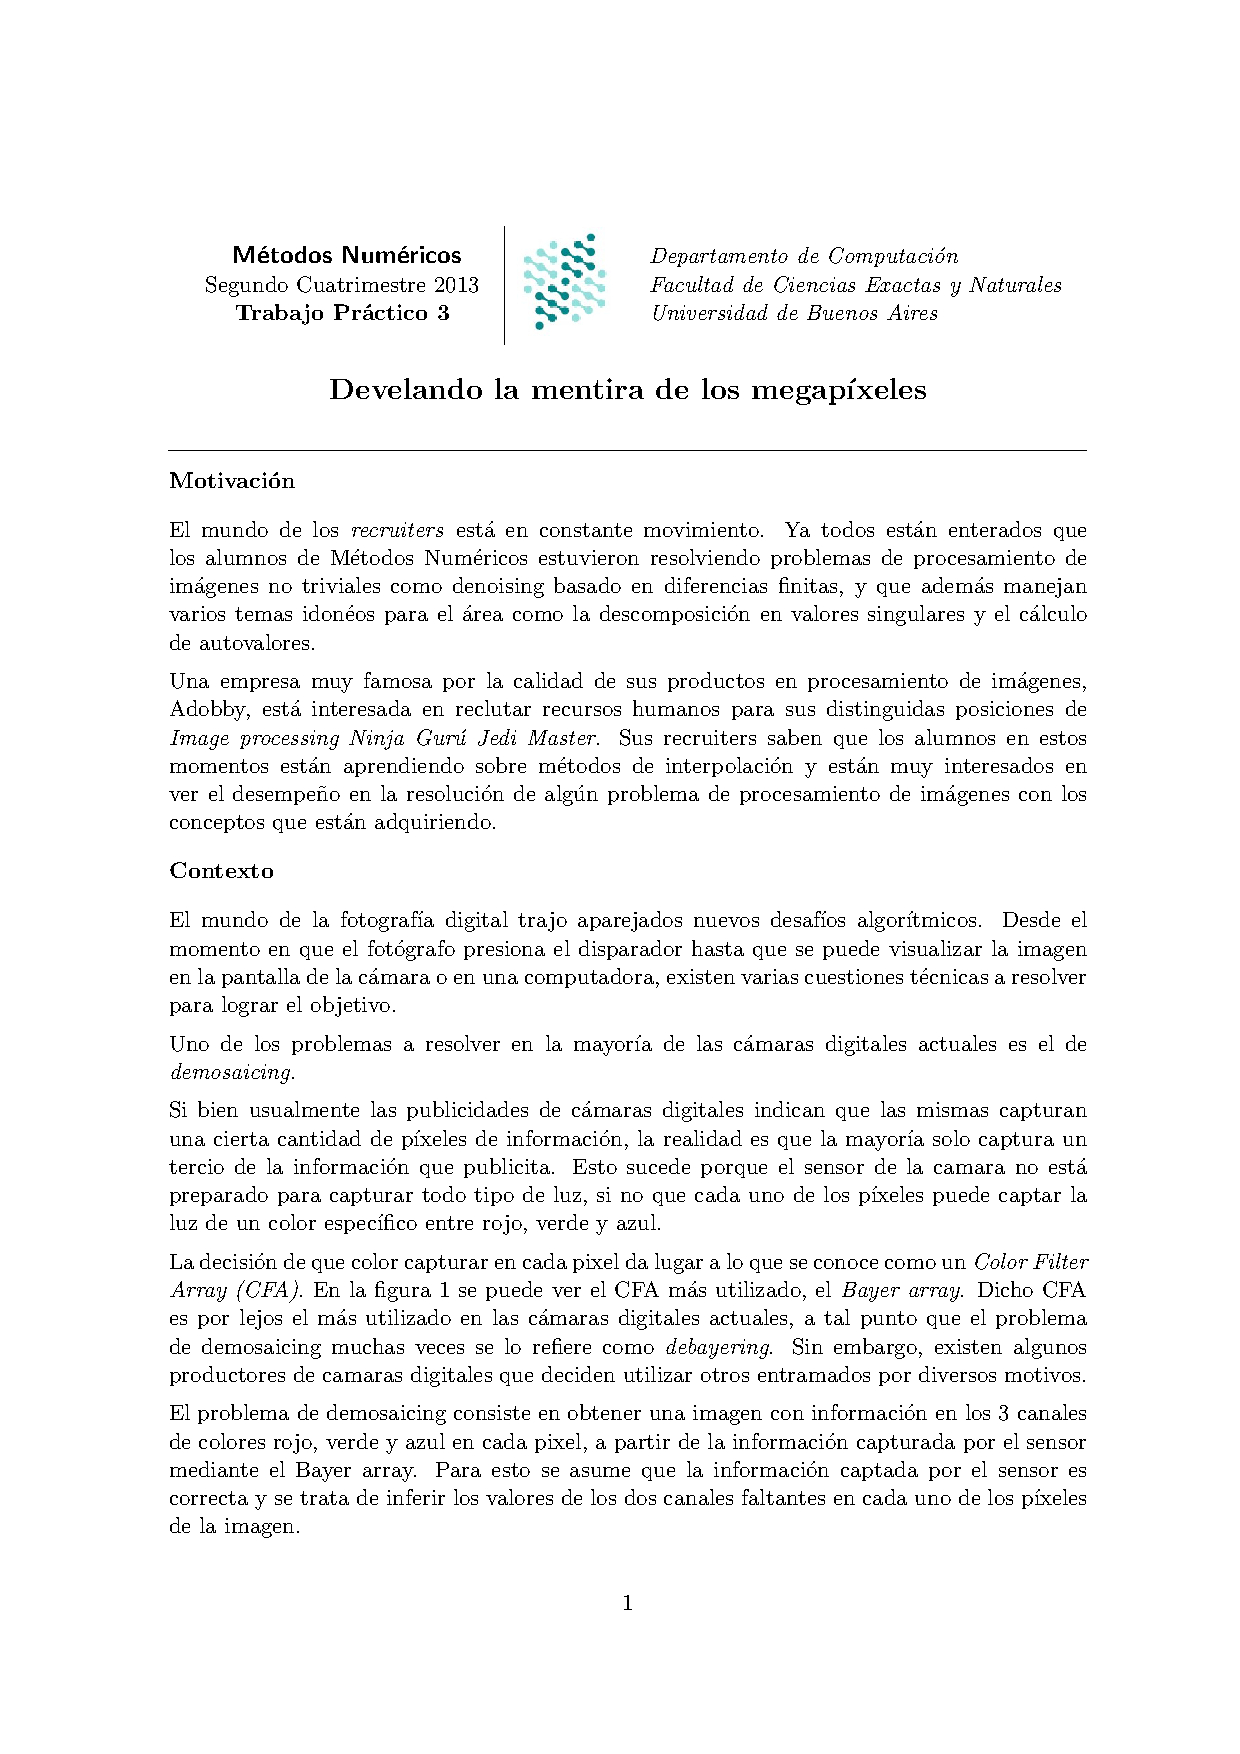
\includepdf[pages={-}]{Enunciado.pdf}

\subsection{Ap\'endice B:}
\newpage
\section{Referencias}
 
\textbf{[1]} Ron Kimmel. Demosaicing: image reconstruction from color ccd samples. \textit{IMAGE PROCESSING, IEEE TRANSACTIONS ON}, 1999. \\
\\

\textbf{[2]} Henrique S. Malvar, Li wei He, and Ross Cutler. High-quality linear interpolation for
demosaicing of bayer-patterned color images. In \textit{Proceedings of the IEEE International
Conference on Speech, Acoustics, and Signal Processing}, 2004.

\end{document}

%%%%%%%%%%%%%%%%%%%%%%%%%%%%%%%%%%%%%%%%%%%%%%%%%%%%%%%%%%%%%%%%%%%%%%%%%
\begin{figure}
  \begin{center}
	
\includegraphics[scale=0.66]{imagenes/logouba.jpg}
	\caption{Descripcion de la figura}
	\label{nombreparareferenciar}
  \end{center}
\end{figure}


\paragraph{\textbf{Titulo del parrafo} } Bla bla bla bla.
Esto se muestra en la figura~\ref{nombreparareferenciar}.



\begin{codesnippet}
\begin{verbatim}

struct Pepe {

    ...

};

\end{verbatim}
\end{codesnippet}
